\documentclass[a4paper,12pt]{article}
%\usepackage[T1]{fontenc} %for å bruke æøå
\usepackage[utf8]{inputenc}
\usepackage{graphicx} %for å inkludere grafikk
\usepackage{subcaption}
%\usepackage{verbatim} %for å inkludere filer med tegn LaTeX ikke liker
\usepackage{tabularx}
%\usepackage{mathpazo}
\usepackage{cancel}
\usepackage[sep=3pt, offset=1.1em]{simpler-wick}
\usepackage{physics}
\usepackage[left=1cm, right=1cm, top=2cm]{geometry}
\usepackage{listings}
%\usepackage{color}
\usepackage{float}
\usepackage{url}
\usepackage{amsmath}
\usepackage{tikz}
\usetikzlibrary{arrows,decorations.markings}

%biblatex
\usepackage[backend=bibtex,
            sorting=ynt]{biblatex}
\addbibresource{refs.bib}

%\definecolor{dkgreen}{rgb}{0,0.6,0}
%\definecolor{gray}{rgb}{0.5,0.5,0.5}
%\definecolor{mauve}{rgb}{0.58,0,0.82}
%\definecolor{darkblue}{rgb}{0.0,0.0,0.6}
%\definecolor{cyan}{rgb}{0.0,0.6,0.6}

\newcommand{\hatH}{\hat{H}}
\newcommand{\hatTt}{\hat{T}_2}
\newcommand{\brak}[2]{\mel{#1}{\hat{v}}{#2}}
\newcommand{\ad}{a^\dagger}
\newcommand{\del}[1]{\delta_{#1}}
\newcommand{\phiijab}{\Phi_{ij}^{ab}}
\newcommand{\Phat}[1]{\hat{P}(#1)}
\newcommand{\bs}[1]{\boldsymbol{{#1}}}
\newcommand{\psin}{\Psi_n(\bs{r})}

\lstset{frame=tb,
  language=Python,
  breaklines=true,
  showstringspaces=false,
  columns=flexible,
  numbers=none,
  identifierstyle=\color{darkblue},
  commentstyle=\color{dkgreen},
  stringstyle=\color{mauve},
  tabsize=3
}
\lstdefinelanguage{XML}
{
  morestring=[b]",
  morestring=[s]{>}{<},
  morecomment=[s]{<?}{?>},
  stringstyle=\color{black},
  identifierstyle=\color{darkblue},
  keywordstyle=\color{cyan},
  morekeywords={xmlns,version,type,ma-id}% list your attributes here
}

\bibliographystyle{abbrv}
\setlength\parindent{0pt}

\title{FYS4480 - Project 2}
\author{Stian Bilek \& Even Nordhagen}

\date{\today}

%\setlength\parindent{0pt}

\begin{document}

\maketitle
\abstract{The aim of this project is to perform a Coupled Cluster Doubles (CCD) implementation from scratch and apply it on ground state energy estimations of Helium and Beryllium. We limit ourselves to the s-waves and let the single-particle orbitals 1s, 2s and 3s form the basis. The obtained energies were compared to energies found using configuration interaction (CI), Hartree-Fock (HF) and second order many-body perturbation theory (MBPT), and we also use the HF-basis as input to CCD.  \iffalse and in that manner this project works as a comparison between the different methods.\fi

The results provided by CCD turned out to be poor using the original basis for both atoms, and it was outperformed by all other methods but MBPT. In fact, the energies were just slightly lower than the reference energies. When moving to HF-basis, the results improved dramatically giving relative errors of 2.22\% and 1.05\% for Helium and Beryllium respectively, compared to the experimental values. With an energy approximation of $-2.839144 [a.u.]$ for Helium and $-14.5129 [a.u.]$ for Beryllium, this approach provided the best results yet.
}

\section{Introduction}
Over the past century, plenty of methods have been developed in order to solve the time independent Schrödinger equation,
\begin{equation*}
\label{eq:schrodinger}
 \hat{H}\psin=\epsilon_n\psin,
\end{equation*}
which is the equation to solve to find the energy of a stationary quantum mechanical system. One of those clever methods is the Coupled Cluster method (CC), which approximates the wave function with an exponential expansion. Actually, this approach is in principle capable of giving the exact results if not limited by computational capacity \cite{crawford}. The method was invented by Fritz Coester and Herman Kümmel during the 1950's, but it was not given that the method would be a success. In his biography, Kümmel writes the following about his thoughts on the situation of coupled cluster in the late fifties \cite{kummel}: \\

''\textit{I myself at the time had almost given up the CC method as not tractable...}''\\\\
As a paradox, the method is today the \textit{de facto} standard wave function-based method for electronic-structure calculations. \cite{paldus}

\bigskip
In this project, we will use Coupled Cluster Doubles (CCD) to estimate the ground state energy of Helium and Beryllium, with and without a Hartree-Fock basis. We will then compare the obtained energies with the experimental values and our previously obtained results for the Configuration Interaction Singles (CIS) and Hartree-Fock (HF) method \cite{project1even}. In section \ref{sec:Theory}, we will introduce the theory and methods used to obtain our results, starting with a representation of our Hamiltonian and basis states in section \ref{subsec:manybodyqt}. We then give a derivation of the CCD energy and amplitude equations, as well as a comparison between this method and CIS in section \ref{sec:CCD} - \ref{sec:CIVSCC}. When we move over to the results section, we represent our results for the Helium and Beryllium atom in section \ref{sec:HeliumResults} and \ref{sec:BerylliumResults}, respectively. In section \ref{sec:Discussion} we will discuss these results and finally conclude them in section \ref{sec:Conclusion}.

We recommend reading the theory section of our previous projects \cite{project1even}\cite{project1stian} as it contains details about CIS, HF and second quantization that are not provided here. 

\section{Theory}
\label{sec:Theory}
\subsection{Many Body Quantum Theory}
\label{subsec:manybodyqt}
With the Hamiltonian we will work with we have introduced the Born-Oppenheimer approximation which effectively freezes our the nucleonic degrees of freedom. For $N$ electrons it has the following form:

$$\hat{H} = \sum_{i=1}^N t(x_i) - \sum_{i=1}^N k\frac{Ze^2}{r_i} + \sum_{i<j}^N \frac{ke^2}{r_{ij}}$$
where $k = 1.44 eVnm$ and $r_{ij} = |r_i - r_j|$. We will introduce atomic units, which means that $c = e = m_e = \hbar = 1$. This makes the constant $k=1$. The energies represented can be multiplied with $2 \times 13.6 eV$ to obtain energies in electron volts. The Hamiltonian can then be rewritten as
\begin{equation}
\label{eq:Hamiltonian}
	\hat{H} = \hat{H}_0 + \hat{H}_1 = \sum_{i = 1}^N \hat{h}(x_i) + \sum_{i<j}^{N} \frac{1}{r_{ij}}
\end{equation}
where $\hat{h} = \hat{t} - \frac{Z}{r_i}$. Thus the Hamiltonian can be represented by a sum over $N$ one body Hamiltonians $\hat{h}(x_i)$ and a sum over $N(N-1)/2$ two body interactions $\frac{1}{r_{ij}}$. 
We will use hydrogen-like single particle functions for our calculations which makes the one body operator $\hat{h}$ diagonal in our basis. The one body expectation values are given by

\begin{equation}
\label{eq:singleparticleEnergies}
\bra{i} \hat{h} \ket{j} = -\frac{Z^2}{2n^2} \delta_{ij}
\end{equation}
where the quantum number $n$ refers to the number of nodes of the wave function. We will restrict ourselves to s-waves, which means that the orbital momentum $l=0$. We will also assume that the total spin projection $M_S = 0$.
In addition, we need to be careful when calculating the expectation values since our wave function is a product of spatial and spin functions. Our Hamiltonian consists of operators that are not dependent on spin, which means that we can integrate over the spin variable separately.

\bigskip
For our one-electron intergrals, this means that
\begin{equation}
\label{eq:spinorthooneelec}
	\bra{\psi_i}\hat{h} \ket{\psi_j} = \bra{i} \hat{h} \ket{j} \bra{\sigma_i}\ket{\sigma_j} = \bra{i} \hat{h} \ket{j} \delta_{\sigma_i \sigma_j}
\end{equation}
where $\ket{\psi_i}$ represents the spin orbitals, $\ket{i}$ represents the spatial part and $\ket{\sigma_i}$ represents the spin part.
\bigskip
For two-electron integrals, we get

\begin{equation}
\label{eq:spinorthotwoelec}
	\bra{\psi_i \psi_j} \hat{v} \ket{\psi_k \psi_l} = \bra{ij} \hat{h} \ket{kl} \bra{\sigma_i}\ket{\sigma_k}\bra{\sigma_j}\ket{\sigma_l} = \bra{ij} \hat{h} \ket{kl} \delta_{\sigma_i \sigma_k} \delta_{\sigma_j \sigma_l}
\end{equation}
\bigskip
The most convenient many-particle wave functions to work with are given by the simple product
$$\Psi(x_1, x_2, \cdots ,x_N)  = \psi_1(x_1)\psi_2(x_2) \cdots \psi_N(x_N)$$
For fermionic systems however, the Pauli exclusion principle requires wave functions to be anti-symmetric under the exchange of two particles. This requirement is satisfied by $\Psi$ being represented by a Slater determinant (SD)
\begin{equation}
\label{eq:SD}
	\Psi(x_1 x_2 \cdots x_N) = \frac{1}{\sqrt{N!}}\begin{vmatrix}
	\psi_1(x_1) & \psi_1(x_2) &\psi_1(x_3) & \dots & \psi_1(x_N) \\ 
	\psi_2(x_1) & \psi_2(x_2) & \psi_2(x_3 & \dots & \psi_2(x_N) \\
	\vdots & \vdots & \vdots & \ddots & \vdots \\
	\psi_N(x_1) & \psi_N(x_2) & \psi_N(x_3) & \dots & \psi_N(x_N)
	\end{vmatrix}
\end{equation}
An important property is that if the set $\{\psi_i\}$ is complete, an arbitrary antisymmetric N-electron wave function can be written as a linear combination of all possible N-electron Slater determinants:

\begin{equation}
\label{eq:SlaterLinearComb}
	\ket{\Phi} = c_0 \ket{\Psi_0} + \sum_{ia} c_i^a \ket{\Psi_i^a} + 					\sum_{i<j,a<b} c_{ij}^{ab} \ket{\Psi_{ij}^{ab}} + \cdots 
\end{equation}
The number of $N$-electron Slater determinants that can be formed from $2K$ spin orbitals is
\begin{equation}
\label{eq:(2K/N)}
	\textit{Number of Slater Determinants} = \binom{2K}{N}
\end{equation}
Given that we are working with the s-waves 1s-3s and electrons, we will have six basis states to work with. We omit the labels $s, l$ and $m_l$, and write our single-particle states as $\psi_{n,m_s}$ with $n$ being the number of nodes of the wave function and $m_s \in \{\uparrow, \downarrow \}$ refers to the secondary spin quantum number. To simplify our notation further, we label our basis states as in table \ref{tab:basisstates} below
\begin{table}[H]
\caption{Basis States}
\centering
\begin{tabular}{cc}
$\ket{1} = \ket{\psi_{1,\uparrow}}$ & $\ket{2} = \ket{\psi_{1,\downarrow}}$ \\[1cm] 
$\ket{3} = \ket{\psi_{2,\uparrow}}$ & $\ket{4} = \ket{\psi_{2,\downarrow}}$ \\[1cm]
$\ket{5} = \ket{\psi_{3,\uparrow}}$ & $\ket{6} = \ket{\psi_{3,\downarrow}}$ 
\label{tab:basisstates}
\end{tabular}
\end{table}
Whenever we use ket notation for a many-particle state in our report, we are referring to a SD. For example, the ket $ \ket{c} $ refers to the reference vacuum SD.

\subsubsection{Helium}
When approximating the ground state of the Helium atom, we will use 
\begin{equation*}
    \ket{c}\equiv\frac{1}{2}\Big[\ket{12}-\ket{21}\Big]\equiv \ket{12}_{\text{AS}}
\end{equation*}
as our reference vacuum, which schematically is represented in figure \ref{fig:schematic_he_gs}, where the hole labels are defined as $ijk... \in \{1,2\}$ and particle labels as $abc... \in \{3,4,5,6\}$. The attribute AS will henceforth be skipped. 
\begin{figure} [H]
	\begin{center}
		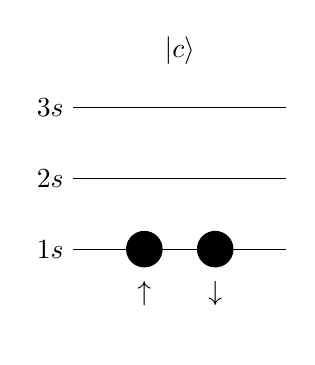
\begin{tikzpicture}[scale=0.9]
		\begin{scope}
			\foreach \i in {1,...,3}
			{
				\draw (-1,\i-1) node[anchor=east] {$\i s$} --(2,\i-1);
			}
			\filldraw (0,0) node[anchor=north,inner sep=.4cm] {$\uparrow$} circle (0.25cm); 
			\filldraw (1,0) node[anchor=north,inner sep=.4cm] {$\downarrow$} circle (0.25cm);
			\node[] at (0.5,2.8) {$\ket{c}$};
		\end{scope}
		\end{tikzpicture}
	\end{center}
\caption{Ground state of Helium.}
\label{fig:schematic_he_gs}
\end{figure}
We also have the excited 1p-1h and 2p-2h states listed in figure \ref{fig:schematic_he}. These states together form our truncated SD basis.
\begin{figure} [H]
	\begin{center}
		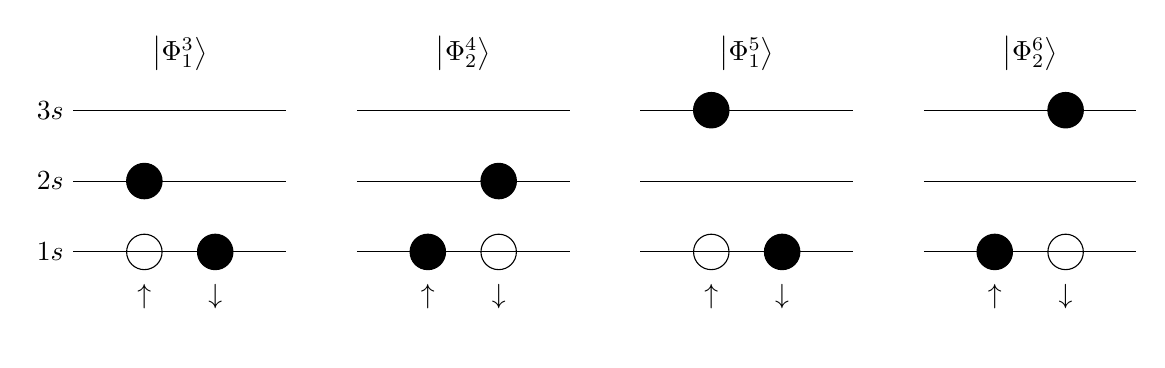
\begin{tikzpicture}[scale=0.9]
		\begin{scope}
		\foreach \i in {1,...,3}
		{
			\draw (-1,\i-1) node[anchor=east] {$\i s$} --(2,\i-1);
		}
		\draw (0,0) node[anchor=north,inner sep=.4cm] {$\uparrow$} circle (0.25cm); 
		\filldraw (1,0) node[anchor=north,inner sep=.4cm] {$\downarrow$} circle (0.25cm);
		\filldraw (0,1) circle (0.25cm);
		\node[] at (0.5,2.8) {$\ket{\Phi_{1}^{3}}$};
		\end{scope}
		\begin{scope}[xshift=4cm]
		\foreach \i in {1,...,3}
		{
			\draw (-1,\i-1) --(2,\i-1);
		}
		\filldraw (0,0) node[anchor=north,inner sep=.4cm] {$\uparrow$} circle (0.25cm); 
		\draw (1,0) node[anchor=north,inner sep=.4cm] {$\downarrow$} circle (0.25cm);
		\filldraw (1,1) circle (0.25cm);
		\node[] at (0.5,2.8) {$\ket{\Phi_{2}^{4}}$};
		\end{scope}
		\begin{scope}[xshift=8cm]
		\foreach \i in {1,...,3}
		{
			\draw (-1,\i-1) --(2,\i-1);
		}
		\draw (0,0) node[anchor=north,inner sep=.4cm] {$\uparrow$} circle (0.25cm); 
		\filldraw (1,0) node[anchor=north,inner sep=.4cm] {$\downarrow$} circle (0.25cm);
		\filldraw (0,2) circle (0.25cm); 
		\node[] at (0.5,2.8) {$\ket{\Phi_{1}^{5}}$};
		\end{scope}
		\begin{scope}[xshift=12cm]
		\foreach \i in {1,...,3}
		{
			\draw (-1,\i-1) --(2,\i-1);
		}
		\filldraw (0,0) node[anchor=north,inner sep=.4cm] {$\uparrow$} circle (0.25cm); 
		\draw (1,0) node[anchor=north,inner sep=.4cm] {$\downarrow$} circle (0.25cm);
		\filldraw (1,2) circle (0.25cm); 
		\node[] at (0.5,2.8) {$\ket{\Phi_{2}^{6}}$};
		\end{scope}
		\end{tikzpicture}
	\end{center}
	\newline
	\begin{center}
		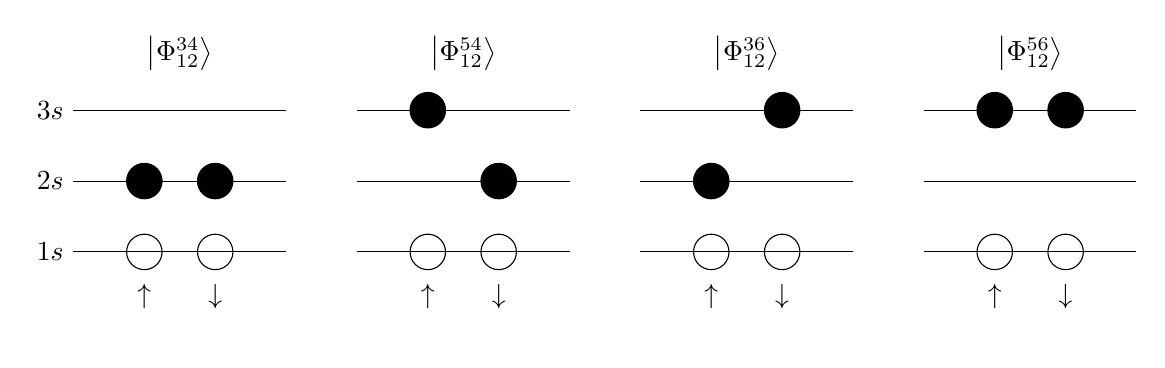
\begin{tikzpicture}[scale=0.9]
		\begin{scope}
		\foreach \i in {1,...,3}
		{
			\draw (-1,\i-1) node[anchor=east] {$\i s$} --(2,\i-1);
		}
		\draw (0,0) node[anchor=north,inner sep=.4cm] {$\uparrow$} circle (0.25cm); 
		\draw (1,0) node[anchor=north,inner sep=.4cm] {$\downarrow$} circle (0.25cm);
		\filldraw (0,1) circle (0.25cm);
		\filldraw (1,1) circle (0.25cm);
		\node[] at (0.5,2.8) {$\ket{\Phi_{12}^{34}}$};
		\end{scope}
		\begin{scope}[xshift=4cm]
		\foreach \i in {1,...,3}
		{
			\draw (-1,\i-1) --(2,\i-1);
		}
		\draw (0,0) node[anchor=north,inner sep=.4cm] {$\uparrow$} circle (0.25cm); 
		\draw (1,0) node[anchor=north,inner sep=.4cm] {$\downarrow$} circle (0.25cm);
		\filldraw (0,2) circle (0.25cm); 
		\filldraw (1,1) circle (0.25cm); 
		\node[] at (0.5,2.8) {$\ket{\Phi_{12}^{54}}$};
		\end{scope}
		\begin{scope}[xshift=8cm]
		\foreach \i in {1,...,3}
		{
			\draw (-1,\i-1) --(2,\i-1);
		}
		\draw (0,0) node[anchor=north,inner sep=.4cm] {$\uparrow$} circle (0.25cm); 
		\draw (1,0) node[anchor=north,inner sep=.4cm] {$\downarrow$} circle (0.25cm);
		\filldraw (1,2) circle (0.25cm);
		\filldraw (0,1) circle (0.25cm);
		\node[] at (0.5,2.8) {$\ket{\Phi_{12}^{36}}$};
		\end{scope}
		\begin{scope}[xshift=12cm]
		\foreach \i in {1,...,3}
		{
			\draw (-1,\i-1) --(2,\i-1);
		}
		\draw (0,0) node[anchor=north,inner sep=.4cm] {$\uparrow$} circle (0.25cm); 
		\draw (1,0) node[anchor=north,inner sep=.4cm] {$\downarrow$} circle (0.25cm);
		\filldraw (0,2) circle (0.25cm); 
		\filldraw (1,2) circle (0.25cm);
		\node[] at (0.5,2.8) {$\ket{\Phi_{12}^{56}}$};
		\end{scope}
		\end{tikzpicture}
	\end{center}
	\caption{Possible states in the 1s, 2s and 3s orbitals of Helium. In the first row, all singly excited states are listed, while in the second row all doubly excited states are listed.}
	\label{fig:schematic_he}
\end{figure}


\subsubsection{Beryllium}
\label{sec:Bery}
For the Beryllium atom, we will use the following state as our reference vacuum SD
\begin{figure} [H]
	\begin{center}
		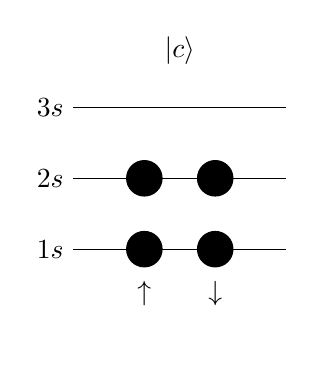
\begin{tikzpicture}[scale=0.9]
		\begin{scope}
		\foreach \i in {1,...,3}
		{
			\draw (-1,\i-1) node[anchor=east] {$\i s$} --(2,\i-1);
		}
		\filldraw (0,0) node[anchor=north,inner sep=.4cm] {$\uparrow$} circle (0.25cm); 
		\filldraw (1,0) node[anchor=north,inner sep=.4cm] {$\downarrow$} circle (0.25cm);
		\filldraw (0,1) circle (0.25cm);
		\filldraw (1,1) circle (0.25cm);
		\node[] at (0.5,2.8) {$\ket{c}$};
		\end{scope}
		\end{tikzpicture}
	\end{center}
	\caption{Ground state of Beryllium.}
	\label{fig:schematic_be_gs}
\end{figure}
which defines our hole labels $ijk... \in \{1,2,3,4\}$ and particle labels $abc... \in \{5,6\}$. The possible 1p-1h and 2p-2h states in our basis are 
\begin{figure} [H]
	\begin{center}
		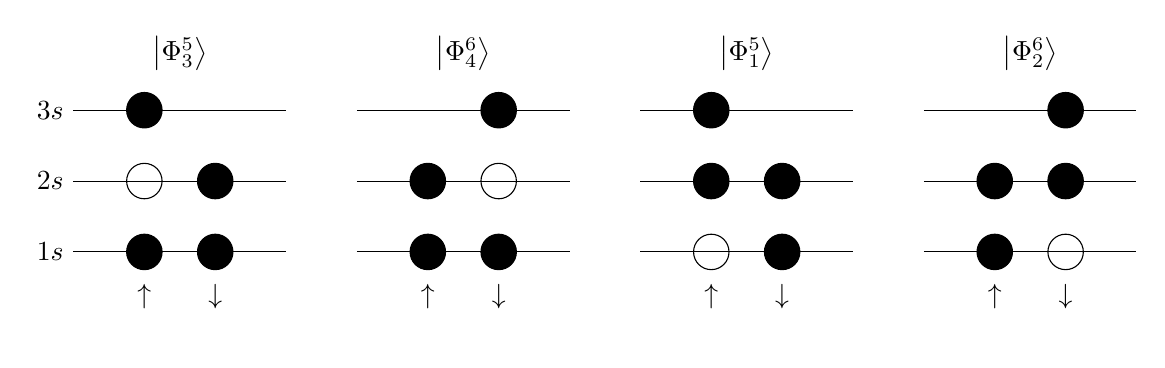
\begin{tikzpicture}[scale=0.9]
		\begin{scope}
		\foreach \i in {1,...,3}
		{
			\draw (-1,\i-1) node[anchor=east] {$\i s$} --(2,\i-1);
		}
		\filldraw (0,0) node[anchor=north,inner sep=.4cm] {$\uparrow$} circle (0.25cm); 
		\filldraw (1,0) node[anchor=north,inner sep=.4cm] {$\downarrow$} circle (0.25cm);
		\draw (0,1) circle (0.25cm);
		\filldraw (1,1) circle (0.25cm);
		\filldraw (0,2) circle (0.25cm);
		\node[] at (0.5,2.8) {$\ket{\Phi_3^5}$};
		\end{scope}
		\begin{scope}[xshift=4cm]
		\foreach \i in {1,...,3}
		{
			\draw (-1,\i-1) --(2,\i-1);
		}
		\filldraw (0,0) node[anchor=north,inner sep=.4cm] {$\uparrow$} circle (0.25cm); 
		\filldraw (1,0) node[anchor=north,inner sep=.4cm] {$\downarrow$} circle (0.25cm);
		\draw (1,1) circle (0.25cm);
		\filldraw (1,2) circle (0.25cm);
		\filldraw (0,1) circle (0.25cm);
		\node[] at (0.5,2.8) {$\ket{\Phi_{4}^{6}}$};
		\end{scope}
		\begin{scope}[xshift=8cm]
		\foreach \i in {1,...,3}
		{
			\draw (-1,\i-1) -- (2,\i-1);
		}
		\draw (0,0) node[anchor=north,inner sep=.4cm] {$\uparrow$} circle (0.25cm); 
		\filldraw (1,0) node[anchor=north,inner sep=.4cm] {$\downarrow$} circle (0.25cm);
		\filldraw (0,1) circle (0.25cm);
		\filldraw (1,1) circle (0.25cm);
		\filldraw (0,2) circle (0.25cm);
		\node[] at (0.5,2.8) {$\ket{\Phi_{1}^{5}}$};
		\end{scope}
		\begin{scope}[xshift=12cm]
		\foreach \i in {1,...,3}
		{
			\draw (-1,\i-1) --(2,\i-1);
		}
		\filldraw (0,0) node[anchor=north,inner sep=.4cm] {$\uparrow$} circle (0.25cm); 
		\draw (1,0) node[anchor=north,inner sep=.4cm] {$\downarrow$} circle (0.25cm);
		\filldraw (1,1) circle (0.25cm);
		\filldraw (1,2) circle (0.25cm);
		\filldraw (0,1) circle (0.25cm);
		\node[] at (0.5,2.8) {$\ket{\Phi_{2}^{6}}$};
		\end{scope}
		\end{tikzpicture}
	\end{center}
	\newline
	\begin{center}
		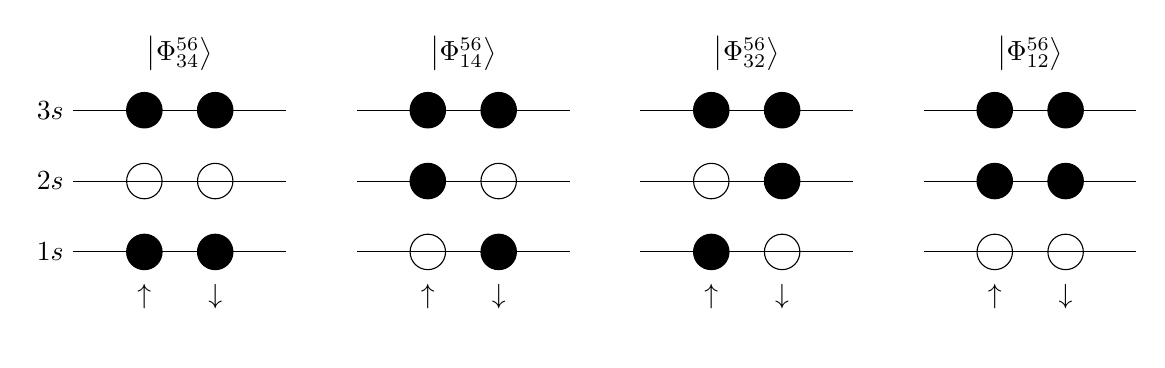
\begin{tikzpicture}[scale=0.9]
		\begin{scope}
		\foreach \i in {1,...,3}
		{
			\draw (-1,\i-1) node[anchor=east] {$\i s$} --(2,\i-1);
		}
		\filldraw (0,0) node[anchor=north,inner sep=.4cm] {$\uparrow$} circle (0.25cm); 
		\filldraw (1,0) node[anchor=north,inner sep=.4cm] {$\downarrow$} circle (0.25cm);
		\draw (0,1) circle (0.25cm);
		\draw (1,1) circle (0.25cm);
		\filldraw (0,2) circle (0.25cm);
		\filldraw (1,2) circle (0.25cm);
		\node[] at (0.5,2.8) {$\ket{\Phi_{34}^{56}}$};
		\end{scope}
		\begin{scope}[xshift=4cm]
		\foreach \i in {1,...,3}
		{
			\draw (-1,\i-1) --(2,\i-1);
		}
		\draw (0,0) node[anchor=north,inner sep=.4cm] {$\uparrow$} circle (0.25cm); 
		\filldraw (1,0) node[anchor=north,inner sep=.4cm] {$\downarrow$} circle (0.25cm);
		\draw (1,1) circle (0.25cm);
		\filldraw (1,2) circle (0.25cm);
		\filldraw (0,2) circle (0.25cm);
		\filldraw (0,1) circle (0.25cm);
		\node[] at (0.5,2.8) {$\ket{\Phi_{14}^{56}}$};
		\end{scope}
		\begin{scope}[xshift=8cm]
		\foreach \i in {1,...,3}
		{
			\draw (-1,\i-1) -- (2,\i-1);
		}
		\filldraw (0,0) node[anchor=north,inner sep=.4cm] {$\uparrow$} circle (0.25cm); 
		\draw (1,0) node[anchor=north,inner sep=.4cm] {$\downarrow$} circle (0.25cm);
		\draw (0,1) circle (0.25cm);
		\filldraw (1,1) circle (0.25cm);
		\filldraw (0,2) circle (0.25cm);
		\filldraw (1,2) circle (0.25cm);
		\node[] at (0.5,2.8) {$\ket{\Phi_{32}^{56}}$};
		\end{scope}
		\begin{scope}[xshift=12cm]
		\foreach \i in {1,...,3}
		{
			\draw (-1,\i-1) --(2,\i-1);
		}
		\draw (0,0) node[anchor=north,inner sep=.4cm] {$\uparrow$} circle (0.25cm); 
		\draw (1,0) node[anchor=north,inner sep=.4cm] {$\downarrow$} circle (0.25cm);
		\filldraw (1,1) circle (0.25cm);
		\filldraw (1,2) circle (0.25cm);
		\filldraw (0,1) circle (0.25cm);
		\filldraw (0,2) circle (0.25cm);
		\node[] at (0.5,2.8) {$\ket{\Phi_{12}^{56}}$};
		\end{scope}
		\end{tikzpicture}
	\end{center}
	\caption{Possible states in the 1s, 2s and 3s orbitals of Beryllium. In the first row, all singly excited states are listed, while in the second row all doubly excited states are listed.}
	\label{fig:schematic}
\end{figure}
Which completes our truncated SD basis.



\subsection{Coupled Cluster Method}
\label{sec:CCD}
In coupled cluster theory, we start out with an ansatz for the ground state

\begin{equation}
    \label{eq:CCTGroundstateAnsatz}
    \ket{\Psi_{CC}} = e^{\hat{T}}\ket{c}
\end{equation}
where $\ket{c}$ is our reference vacuum and $\hat{T}$ is the cluster operator
$$\hat{T} = \hat{T}_1 + \hat{T}_2 + \cdots $$
$$\hat{T}_n = \left( \frac{1}{n!}\right)^2 \sum_{abc...} \sum_{ijk...} t_{ijk...}^{abc...}a^\dagger_aa_b^\dagger a_c^\dagger \cdots a_ka_ja_i$$
In our project, we will limit ourselves to Coupled Cluster Doubles (CCD), which makes our cluster operator

\begin{equation}
    \label{eq:CCDOperator}
    \hat{T} = \hat{T}_2 = \frac{1}{4}\sum_{ab} \sum_{ij} t_{ij}^{ab}a^\dagger_a a^\dagger_b a_j a_i 
\end{equation}
The Schrödinger equation becomes 

\begin{equation}
    \label{eq:SE}
    \hat{H}\ket{\Psi_{CC}} = E_{CC}\ket{\Psi_{CC}} \qquad \hat{H} e^{\hat{T}}\ket{c} = E_{CC} e^{\hat{T}}\ket{c}
\end{equation}
If we left multiply this equation with $\bra{c} e^{-\hat{T}}$, we get

$$\bra{c}e^{-\hat{T}} \hat{H} e^{\hat{T}} \ket{c} = E_{CC}\bra{c} e^{-\hat{T}}e^{\hat{T}} \ket{c} = E_{CC}$$
Which we write in terms of the similarity transformed Hamiltonian $\overline{H} = e^{-\hat{T}} \hat{H} e^{\hat{T}}$:

\begin{equation}
    \bra{c} \overline{H} \ket{c} = E_{CC}
\end{equation}
In the same manner, we can left multiply the Schrödinger equation with $e^{-\hat{T}} \ket{\Phi_{ij...}^{ab...}}$ to obtain
\begin{equation}
    \label{eq:CCTsolv}
    \mel{\Phi_{ij...}^{ab...}}{\overline{H}}{c} = 0
\end{equation}
Equation \ref{eq:CCTsolv} can be used to find the unknowns $t^{abc...}_{ijk...}$. To do this, we can expand our Coupled Cluster Hamiltonian using the Baker-Campbell-Hausdorff expansion

\begin{align}
    \label{eq:BCH}
    \overline{H} = \hat{H} &+ [\hat{H},\hat{T}]\notag \\
                        &+ \frac{1}{2}[[\hat{H},\hat{T}],\hat{T}]\notag \\
                        &+ \frac{1}{6}[[[\hat{H},\hat{T}],\hat{T}],\hat{T}] \\
                        &+ \frac{1}{24}[[[[\hat{H},\hat{T}],\hat{T}],\hat{T}],\hat{T}] \notag \\
                        &+ \cdots \notag
\end{align}
where our Hamiltonian $\hat{H}$ is given by 
\begin{align}
    \label{eq:hamiltonian}
    \hatH &=E_{\text{ref}}+\hat{F} + \hat{H}_I \notag \\
         &= E_{\text{ref}} + \sum_{pq}\bra{p}\hat{f} \ket{q} \{a^\dagger_p a_q \} + \frac{1}{4}\sum_{pqrs} \brak{pq}{rs} \{a^\dagger_p a^\dagger_q a_s a_r \}
\end{align}


\subsubsection{Energy equations} \label{sec:energy}
To calculate the coupled cluster energy, we need to solve
\begin{equation}
    E=\mel{c}{\bar{H}}{c}
    \label{eq:ccenergy}
\end{equation}
where $\bar{H}$ is the similarity transformed Hamiltonian described above. Inserting Baker-Campbell-Hausdorff expansion (eq. \ref{eq:BCH}), we get
\begin{equation}
    E=\mel{c}{\hat{H}}{c}+\mel{c}{[\hatH,\hat{T_2}]}{c}+\frac{1}{2}\mel{c}{[[\hatH,\hat{T_2}],\hat{T_2}]}{c}+\text{higher order terms}
\end{equation}
where the Hamiltonian is given by eq. \ref{eq:hamiltonian}.
From Wick's generalized theorem, we immediately see that the first term is the reference energy,
\begin{equation}
    \mel{c}{\hat{H}}{c}=E_{\text{ref}}.
\end{equation}
Further, the second term can be split up into four terms
\begin{equation}
    \mel{c}{[\hatH,\hat{T_2}]}{c}=\mel{c}{\hat{F}\hat{T_2}}{c}-\mel{c}{\hat{T_2}\hat{F}}{c}+\mel{c}{\hat{H}_I\hat{T_2}}{c}-\mel{c}{\hat{T_2}\hat{H}_I}{c}
\end{equation}
where the two former terms obviously do not contribute due to lack of full contractions. The third term can be calculated using Wicks's theorem:
\begin{align}
    \mel{c}{\hat{H}_I\hat{T_2}}{c}&=\frac{1}{16}\sum_{pqrs}\sum_{abij}t_{ij}^{ab}\brak{pq}{rs}\mel{c}{\{a_p^{\dagger}a_q^{\dagger}a_sa_r\}\{a_a^{\dagger}a_b^{\dagger}a_ja_i\}}{c}\\
    &=\frac{1}{16}\sum_{pqrs}\sum_{abij}t_{ij}^{ab}\brak{pq}{rs}\Big(\delta_{pi}\delta_{qj}\delta_{sb}\delta_{ra}-\delta_{pi}\delta_{qj}\delta_{sa}\delta_{rb}+\delta_{pj}\delta_{qi}\delta_{sa}\delta_{rb}-\delta_{pj}\delta_{qi}\delta_{sb}\delta_{ra}\Big)\\
    &=\frac{1}{4}\sum_{abij}t_{ij}^{ab}\brak{ij}{ab}.
\end{align}
Finally, the last term becomes zero because it has a creation operator acting on the bra, which means that 
\begin{equation}
    \mel{c}{[\hatH,\hat{T_2}]}{c}=\frac{1}{4}\sum_{abij}t_{ij}^{ab}\brak{ij}{ab}.
\end{equation}
The last term in the energy expression can be simplified
\begin{align}
    \mel{c}{[[\hatH,\hat{T}_2], \hat{T}_2]}{c}&=\mel{c}{[(\hatH\hatTt-\hatTt\hatH),\hatTt]}{c}\notag\\
    &=\mel{c}{(\hatH\hatTt^2-\hatTt\hatH\hatTt+\hatTt\hatH\hatTt-\hatTt^2\hatH)}{c}\notag\\
    &=\mel{c}{(\hatH\hatTt^2-\hatTt^2\hatH)}{c}.
\end{align}
This is zero since our Slater determinants (SD) are orthogonal and $\hatTt^2$ creates 4p-4h states, while the Hamiltonian is only able to create two 2p-2h states. The fully CCD energy then reads

\begin{equation}
\label{eq:CCDENERGY}
E_{\text{CCD}}=E_{\text{ref}}+\frac{1}{4}\sum_{abij}t_{ij}^{ab}\brak{ij}{ab}
\end{equation}

\subsubsection{Amplitude equations}
We now need to solve for $t_{ij}^{ab}$ in order to find the CCD energy given above. This can be done by first finding an algebraic expression for the amplitude equation (eq. \ref{eq:CCTsolv}). By using eq. \ref{eq:BCH}, we get
\begin{align}
    \label{eq:AMPeqHamil}
    \bra{\Phi_{ij}^{ab}} \overline{H} \ket{c} &= \bra{\Phi_{ij}^{ab}} \hat{H} \ket{c} \notag \\
    & + \bra{\Phi_{ij}^{ab}} [\hat{H},\hat{T}_2] \ket{c} \notag \\
     &+ \frac{1}{2} \bra{\Phi_{ij}^{ab}} [[\hat{H},\hat{T}_2],\hat{T}_2] \ket{c} \\
     &+ \frac{1}{6} \bra{\Phi_{ij}^{ab}} [[[\hatH,\hatTt],\hatTt],\hatTt] \ket{c} \notag \\
     &+ \cdots \notag 
\end{align}
where $\hat{H}$ is still given by eq. \ref{eq:hamiltonian}. The first expression to the right of the equal sign can be broken into three parts. The first:
$$\bra{\Phi_{ij}^{ab}} E_{\textit{ref}} \ket{c} = 0$$
because of the orthogonality of our SDs. Next up is
$$\bra{\Phi_{ij}^{ab}} \hat{F} \ket{c} = 0$$
for the same reason ($\hat{F}$ is only able to create 1p-1h on the reference vacuum). This is known as the Slater-Condon rule.
The final can be simplified using Wicks generalized theorem:
\begin{align*}
\mel{\Phi_{ij}^{ab}}{\har{H}_I}{c} &= \frac{1}{4} \sum_{pqrs}\brak{pq}{rs} \bra{c}a^\dagger_i a^\dagger_j a_b a_a \{a^\dagger_p a^\dagger_q a_s a_r \} \ket{c}\\
&
\begin{aligned}
=\frac{1}{4}\sum_{pqrs}\brak{pq}{rs}(&\delta_{ir}\delta_{js}\delta_{ap}\delta_{bq} - \delta_{si}\delta_{jr}\delta_{bq}\delta_{ap} + \\ & \delta_{si}\delta_{jr}\delta_{bp}\delta_{aq} - \delta_{ir}\delta_{js}\delta_{bp}\delta_{aq})
\end{aligned} \\
& = \brak{ab}{ij}
\end{align*}
The second term in eq. \ref{eq:AMPeqHamil} can be split into six parts, 
\begin{align*}
    \mel{\Phi_{ij}^{ab}}{[\hatH,\hat{T_2}]}{c} &= \mel{\Phi_{ij}^{ab}}{E_{ref}\hatTt}{c} - \mel{\Phi_{ij}^{ab}}{\hatTt E_{ref}}{c} \\ &+ \mel{\Phi_{ij}^{ab}}{\hat{F}\hat{T_2}}{c}-\mel{\Phi_{ij}^{ab}}{\hat{T_2}\hat{F}}{c}\\
    &+\mel{\Phi_{ij}^{ab}}{\hat{H}_I\hat{T_2}}{c}-\mel{\Phi_{ij}^{ab}}{\hat{T_2}\hat{H}_I}{c}
\end{align*}


The first two terms obviously cancel out. The third term can again be calculated using Wick's generalized theorem. The result is
\begin{equation}
    \mel{\phiijab}{\hat{F}\hatTt}{c}=\sum_kf_i^kt_{jk}^{ab}\Phat{ij}-\sum_cf_c^at_{ij}^{bc}\Phat{ab},
\end{equation}
which is shown in Appendix A. The operator $\Phat{pq}$ gives the current term minus a similar term with indices $p$ and $q$ switched,
\begin{equation}
    \Phat{pq}=1-\hat{P}_{pq}
\end{equation}
where $\hat{P}_{pq}$ permutes the indices $p$ and $q$.

Now to the second and last term

\begin{equation}
\mel{\Phi_{ij}^{ab}}{\hat{H}_I\hat{T_2}}{c} = \frac{1}{16} \sum_{cd} \sum_{kl} t_{kl}^{cd} \sum_{pqrs} \bra{c} \ad_i \ad_j a_b a_a \{\ad_p \ad_q a_s a_r \} \ad_c \ad_d a_l a_k \ket{c}
\end{equation}
By using Wicks generalized theorem we see that this can be written as
\begin{equation}
\mel{\Phi_{ij}^{ab}}{\hat{H}_I\hat{T_2}}{c} = \frac{1}{2} \sum_{cd} t_{ij}^{cd}\brak{ab}{cd} + \frac{1}{2} \sum_{kl} t_{kl}^{ab} \brak{kl}{ij} + \hat{P}(ab)\hat{P}(ij)\sum_{kc}t_{jk}^{bc}\brak{ak}{ic}
\end{equation}
because of the anti-symmetry of $t_{kl...}^{cd...}$ and the anti-symmetry of the matrix elements. The derivation is given in appendix A. The final term of eq. \ref{eq:AMPeqHamil} will be zero since we have the normal ordered terms of the Hamiltonian next to the reference vacuum ket.\newline
For the third term in eq. \ref{eq:AMPeqHamil} we proceed in the same manner. First we have
\begin{equation*}
    \mel{\Phi_{ij}^{ab}}{[[E_{ref},\hatTt],\hatTt]}{c} = 0
\end{equation*}
since $E_{ref}$ is a constant. Next we have
\begin{equation*}
    \mel{\Phi_{ij}^{ab}}{[[\hat{F},\hatTt],\hatTt]}{c} = \mel{\Phi_{ij}^{ab}}{(\hat{F}\hatTt^2 - \hatTt^2\hat{F})}{c} = 0
\end{equation*}
since $\hatTt^2$ creates 4p-4h while $\hat{F}$ is a one-body operator.
Finally we have
\begin{equation*}
    \mel{\Phi_{ij}^{ab}}{[[\hat{H}_I,\hatTt],\hatTt]}{c} = \mel{\Phi_{ij}^{ab}}{\hat{H}_I\hatTt^2}{c} - \mel{\Phi_{ij}^{ab}}{\hatTt^2 \hat{H}_I}{c}
\end{equation*}
where the final term becomes zero since $\hat{H}_I$ is normal ordered. We then have
\begin{align*}
    \frac{1}{2}\mel{\Phi_{ij}^{ab}}{[[\hat{H}_I,\hatTt],\hatTt]}{c} = \frac{1}{2}\mel{\Phi_{ij}^{ab}}{\hat{H}_I\hatTt^2}{c} =& \frac{1}{4} \sum_{klcd}\brak{kl}{cd}t_{kl}^{ab}t_{ij}^{cd}\\
    -& \frac{1}{2}\hat{P}(ij) \sum_{klcd} \brak{kl}{cd}t^{ab}_{il}t^{cd}_{kj}\\
    -& \hat{P}(ab)\sum_{klcd}\brak{kl}{cd}t_{ik}^{ac}t_{lj}^{bd}\\
    -&\frac{1}{2}\hat{P}(ab)\sum_{klcd}\brak{kl}{cd}t_{ij}^{ac}t_{kl}^{bd}
\end{align*}


All the subsequent terms of eq. \ref{eq:AMPeqHamil} will be zero. This can be explained by the fact that the n'th term will contain $\hatTt^{n - 1}$, which for $n\geq4$ will result in zero due to the Slater-Condon rules.

Collecting all the terms finally gives
\begin{align*}
    \mel{\Phi_{ij}^{ab}}{\overline{H}}{c} &= \brak{ab}{ij} + \hat{P}(ij)\sum_k f_i^k t_{jk}^{ab} - \hat{P}(ab)\sum_c f_c^a t_{ij}^{bc} \\
    &+ \frac{1}{2}\sum_{kl} \brak{kl}{ij}t^{ab}_{kl} + \hat{P}(ab)\hat{P}(ij) \sum_{kc} \brak{ak}{ic}t_{jk}^{bc} \\
    &+ \frac{1}{2}\sum_{cd} \brak{ab}{cd}t^{cd}_{ij} + \frac{1}{4} \sum_{klcd}\brak{kl}{cd}t_{kl}^{ab}t_{ij}^{cd} - \frac{1}{2}\hat{P}(ij) \sum_{klcd} \brak{kl}{cd}t^{ab}_{il}t^{cd}_{kj} \\
    &- \hat{P}(ab)\sum_{klcd}\brak{kl}{cd}t_{ik}^{ac}t_{lj}^{bd} - \frac{1}{2}\hat{P}(ab)\sum_{klcd}\brak{kl}{cd}t_{ij}^{ac}t_{kl}^{bd} = 0
\end{align*}
By observing that 
$$\hat{P}(ij)\sum_k f_i^k t_{jk}^{ab} = \hat{P}(ij)f_i^i t_{ji}^{ab} + \hat{P}(ij)\sum_{k\neq i} f_i^k t_{jk}^{ab} =  -f_i^i t_{ij}^{ab} - f_j^j t_{ij}^{ab} + \hat{P}(ij)\sum_{k\neq i} f_i^k t_{jk}^{ab} $$
and that
$$\hat{P}(ab)\sum_c f_c^at_{ij}^{bc} = \hat{P}(ab)f_a^at_{ij}^{ba} + \hat{P}(ab)\sum_{c \neq a} f_c^a t_{ij}^{bc} = -f_a^at_{ij}^{ab} - f_b^bt_{ij}^{ab} + \hat{P}(ab)\sum_{c \neq a} f_c^a t_{ij}^{bc}$$
we can rewrite the above equation as
\begin{align}
    \label{eq:AmplitudeIterative}
    t_{ij}^{ab}D_{ab}^{ij} &= \brak{ab}{ij} + \hat{P}(ij)\sum_{k \neq i} f_i^k t_{jk}^{ab} - \hat{P}(ab)\sum_{c \neq a} f_c^a t_{ij}^{bc} \notag \\
    &+ \frac{1}{2}\sum_{kl} \brak{kl}{ij}t^{ab}_{kl} + \hat{P}(ab)\hat{P}(ij) \sum_{kc} \brak{ak}{ic}t_{jk}^{bc} \notag \\
    &+ \frac{1}{2}\sum_{cd} \brak{ab}{cd}t^{cd}_{ij} + \frac{1}{4} \sum_{klcd}\brak{kl}{cd}t_{kl}^{ab}t_{ij}^{cd} - \frac{1}{2}\hat{P}(ij) \sum_{klcd} \brak{kl}{cd}t^{ab}_{il}t^{cd}_{kj} \\
    &- \hat{P}(ab)\sum_{klcd}\brak{kl}{cd}t_{ik}^{ac}t_{lj}^{bd} - \frac{1}{2}\hat{P}(ab)\sum_{klcd}\brak{kl}{cd}t_{ij}^{ac}t_{kl}^{bd} \notag
\end{align}
with $D_{ab}^{ij} = f_i^i + f_j^j - f_a^a - f_b^b$. Dividing the above equation by this factor, we can find $t_{ij}^{ab}$ with an iterative process. Defining the initial guess as
\begin{equation}
    \label{eq:initamplitude}
    t_{ij}^{ab(0)} = \frac{\brak{ab}{ij}}{D_{ab}^{ij}}
\end{equation}
we see by inserting this into the CCD energy equation \ref{eq:CCDENERGY} that we get the second-order perturbation theory energy expression
\begin{equation}
    \label{eq:MBPTEnergy}
    E_{CCD} = E_{ref} + \frac{1}{4} \sum_{abij} \frac{\brak{ab}{ij} \brak{ij}{ab}}{D_{ab}^{ij}}
\end{equation}
Furthermore, if the single particle functions are given by the Hartree-Fock solution
$$\ket{i} = \sum_\alpha C_{i\alpha} \ket{\alpha} $$
where $\ket{\alpha}$ is our orthonormal single particle basis, we see that
\begin{equation*}
    \hat{P}(ij)\sum_{k \neq i} f_i^k t_{jk}^{ab} - \hat{P}(ab)\sum_{c \neq a} f_c^a t_{ij}^{bc} = 0
\end{equation*}
since the Hartree Fock basis functions are the eigenfunctions of the Fock matrix $f_p^q$ and $f_p^q$ will hence be diagonal in this basis.


\subsection{Configuration Interaction vs. Coupled Cluster}
\label{sec:CIVSCC}
For Configuration interaction theory, we use a linear excitation operator for our wave function ansatz
\begin{equation*}
    \Psi^{CI} = (1+ \hat{C})\ket{c} = (1 + \hat{C}_1 + \hat{C}_2 + \cdots)\ket{c}
\end{equation*}
where $\hat{C}_1$ is a single excitation operator, $\hat{C}_2$ is a double excitation operator, etc.
In our task, we will restrict ourselves to the CIS approximation, which means that the ansatz for the ground state energy will be
\begin{equation*}
    \Psi^{CIS} = (1 + \hat{C}_1)\ket{c}
\end{equation*}
For Coupled Cluster theory however, we instead use the expression
\begin{equation*}
    \Psi^{CC} = (1 + \hat{T}_1 + \frac{1}{2!}\hat{T}_1^2 + \frac{1}{3!}\hat{T}_1^3 + \hat{T}_2 + \frac{1}{2!}\hat{T}_2^2 + \cdots)\ket{c}
\end{equation*}
where just like with CI, $\hat{T}_1$ is a single excitation operator, $\hat{T}_2$ is a double excitation operator, etc. The above expression matches that of a power series expansion of an exponential function, which is the reason for the expression in eq. \ref{eq:CCTGroundstateAnsatz}. 
We will also limit ourselves to the CCD approximation, and we will therefore in this case end up with the following ansatz for the ground state
\begin{equation*}
    \Psi^{CCD} = (1 + \hat{T}_2 + \frac{1}{2}\hat{T}_2^2)\ket{c}
\end{equation*}
The above expression implicitly includes higher excitation levels than doubles as we are dealing with the inclusion of $\hat{T}_2^2$ \cite{crawford}.

\section{Results} \label{sec:results}
In Project 1 we estimated the ground state energy of Helium and Beryllium using Configuration Interaction (CI) and Hartree-Fock (HF), and in this project we have added Coupled Cluster Doubles with and without Hartree-Fock basis to our toolbox. For comparison, the results from Project 1 are included with reference to \cite{project1even} and \cite{project1stian}, and we also add the energy from second order perturbation theory (MBPT), which is our initial guess (eq. \ref{eq:MBPTEnergy}). 


\subsection{The Helium atom}
\label{sec:HeliumResults}
\begin{table} [H]
	\caption{Ground state energy of the Helium atom calculated using Configuration Interaction Singles (CIS), Hartree-Fock (HF), second order Many-body Perturbation theory (MBPT) and Coupled Cluster Doubles (CCD). The latter was calculated with and without HF-basis.}
	\begin{tabularx}{\textwidth}{X|X|X} \hline\hline
		\textbf{Method}&\textbf{Energy} [a.u.]&\textbf{Relative error}\\ \hline
		Experimental & -2.903694 & 0.00\%  \\
		Reference & -2.750000 & 5.29\% \\
		CIS & -2.838648 &  2.24\% \\
		HF$_{\text{1 iteration}}$ & -2.829193 & 2.56\% \\
		HF$_{\text{converge}}$ & -2.831096 & 2.50\% \\
		MBPT$_{\text{2nd order}}$ & -2.751508 & 5.24\% \\
		E$_{\text{CCD}}$ & -2.751408 & 5.24\% \\
		E$_{\text{CCD, HF-basis}}$ & -2.839144 & 2.22\% \\ \hline\hline
	\end{tabularx}
	\label{tab:gs_he}
\end{table}


\subsection{The Beryllium atom}
\label{sec:BerylliumResults}
\begin{table} [H]
	\caption{Ground state energy of the Beryllium atom calculated using Configuration Interaction Singles (CIS), Hartree-Fock (HF), second order Many-body Perturbation theory (MBPT) and Coupled Cluster Doubles (CCD). The latter was calculated with and without HF-basis.}
	\begin{tabularx}{\textwidth}{X|X|X} \hline\hline
		\textbf{Method}&\textbf{Energy} [a.u.]&\textbf{Relative error}\\ \hline
		Experimental & -14.6674 & 0.00\%  \\
		Reference & -13.7160 & 6.49\% \\
		CIS & -14.3621 &  2.08\% \\
		HF$_{\text{1 iteration}}$ &  -14.4998 & 1.14\% \\
		HF$_{\text{converge}}$ & -14.5083 & 1.08\% \\
		MBPT$_{\text{2nd order}}$ & -13.7174 & 6.47\% \\
		E$_{\text{CCD}}$ & -13.7211 & 6.45\% \\
		E$_{\text{CCD, HF-basis}}$ & -14.5129 & 1.05\% \\ \hline\hline
	\end{tabularx}
	\label{tab:gs_be}
\end{table}

\section{Discussion}
\label{sec:Discussion}

As we can see from both the results for Helium and for Beryllium, table \ref{tab:gs_he} and table \ref{tab:gs_be} respectively, the CCD method with our single particle basis did not provide better results than our previous calculations. The relative error of $5.24\%$ for Helium with respect to the experimental value is only a slight improvement over the reference vacuum expectation value, which provided a relative error of $5.29\%$.  It is also worth noting that our initial guess, which corresponds to second order MBPT, provided an estimate closer to the experimental results than when letting the CCD algorithm converge. For the Beryllium atom, we got a relative error of $6.45\%$ which is still not great when compared to the other results and compared to the relative error of $6.49\%$ for the reference vacuum expectation value. However, letting the algorithm converge did provide a slightly better estimate than for MBPT, which had a relative error of $6.47\%$. Subsection \ref{sec:CIVSCC} states an important fact that could explain the underwhelming results of CCD. We would expect this method to perform well since it implicitly contains higher order excitations than doubles. However, since our basis (see table \ref{tab:basisstates}) only contains six states, we will not be able to make use of this property as Helium only has two electrons to excite and Beryllium only has two available particle states to excite to. The results of CIS for both Helium and Beryllium being more accurate, with a relative error of $2.24\%$ and $2.08\%$ respectively, seems to therefore suggest that the single excitations are more important in these cases than the double excitations. We would expect CCSD to perform better and it would be interesting to implement this method in later studies.

\bigskip

When instead using CCD with the Hartree-Fock basis, we achieved a much better result. For the Helium atom we beat the current champion, the CIS method and got an energy estimate of $E^{CCD}_{HF} = -2.839144 [a.u]$. This is a slight improvement over CIS, which gave the approximation $E^{CIS} = -2.838648 [a.u]$, but it is an improvement none the less. For the Beryllium atom we also beat the current champion, the Hartree-Fock method and got the energy $E^{CCD}_{HF} = -14.5129 [a.u]$. This is also a slight improvement over as Hartree-Fock gave $E_{HF} = -14.4998 [a.u]$. We expected the CCD method to improve when introducing the HF basis as we replace the reference energy in eq. \ref{eq:CCDENERGY} by the Hartree-Fock energy, HF$_{\text{converge}}$, which is significantly lower. We expected the correction term to give an even better result, which is exactly what happened.

\section{Conclusion}
\label{sec:Conclusion}

When compared to our obtained energies for HF and CIS, we did not see an improvement with the CCD method using our single particle basis for either of the atoms. The results were in fact just a minor enhancement when compared to the reference vacuum expectation value. We argued that the underwhelming results were due to the fact that our basis only included six states, and the implicit inclusion of higher excitation levels than doubles in the CCD method would therefore not be exploited.

However, when switching over to the HF basis we obtained a drastic improvement. For both Helium and Beryllium, the CCD method with the HF basis gave the best results yet with an energy of $-2.839144 \quad [a.u.]$ and $-14.5129 \quad [a.u.]$, respectively. This was in agreement with our expectations as the reference energy in equation \ref{eq:CCDENERGY} is replaced by the HF energy, which is already a significantly better approximation.

\newpage
\appendix
\section{Appendix A} \label{sec:appendixa}
Expression for energy of ground state.

\newpage
\nocite{*}
\printbibliography
\end{document}

